\documentclass[12pt, twoside]{article}
\usepackage[letterpaper, margin=1in, headsep=0.5in]{geometry}
\usepackage[english]{babel}
\usepackage[utf8]{inputenc}
\usepackage{amsmath}
\usepackage{amsfonts}
\usepackage{amssymb}
\usepackage{tikz}
\usetikzlibrary{quotes, angles}
\usepackage{graphicx}
%\usepackage{pgfplots}
%\pgfplotsset{width=10cm,compat=1.9}
%\usepgfplotslibrary{statistics}
%\usepackage{pgfplotstable}
%\usepackage{tkz-fct}
%\usepackage{venndiagram}
\usepackage{enumitem}
\usepackage{multicol}

\usepackage{fancyhdr}
\pagestyle{fancy}
\renewcommand{\headrulewidth}{0pt} % disable the underline of the header

\fancyhead[RO]{Name: \hspace{1.5in}}
\lhead{BECA / Dr. Huson / 10th Grade Geometry\\* 6 December 2018}

\begin{document}
\subsubsection*{Do Now: Triangle congruence proofs}
 \begin{enumerate}
   \item The transversal $\overleftrightarrow{MPR}$ intersects two parallel lines,  $\overleftrightarrow{PQ} || \overleftrightarrow{MN}$. Given $\angle PRQ \cong \angle MPN$ and $P$ bisects $\overline{MR}$. \\Prove $\triangle MPN \cong \triangle PRQ$.
     \begin{center}
     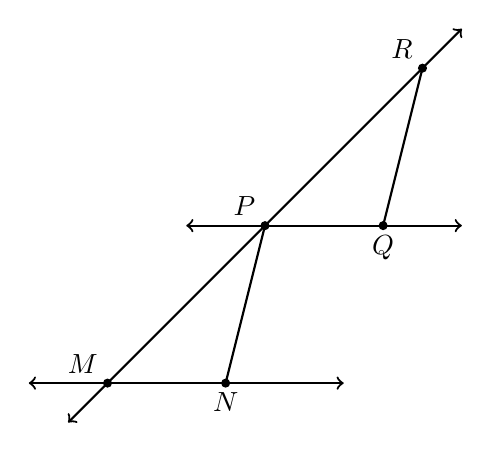
\begin{tikzpicture}[scale=1.0]
       \draw [<->, thick] (-1,0)--(0,0)--(3,0);
       \draw [<->, thick] (-0.5,-0.5)--(4,4)--(4.5,4.5);
       \draw [<->, thick] (1,2)--(4.5,2);
       \draw [-, thick] (4,4)--(3.5, 2);
       \draw [-, thick] (2,2)--(1.5,0);
       \draw [fill] (4,4) circle [radius=0.05] node[above left]{$R$};
       \draw [fill] (3.5, 2) circle [radius=0.05] node[below]{$Q$};
       \draw [fill] (2,2) circle [radius=0.05] node[above left]{$P$};
       \draw [fill] (0,0) circle [radius=0.05] node[above left]{$M$};
       \draw [fill] (1.5,0) circle [radius=0.05] node[below]{$N$};
     \end{tikzpicture}
     \end{center}
     \begin{multicols}{2}
       \underline{Statement} \\
       \underline{Reason}
     \end{multicols}
     \begin{multicols}{2}
       \raggedcolumns
       \begin{enumerate}[label={\arabic*)}]
         \item \rule{4cm}{0.15mm} \vspace{0.3cm}
         \item \rule{4cm}{0.15mm} \vspace{0.3cm}
         \item \rule{4cm}{0.15mm} \vspace{0.3cm}
         \item $\angle RPQ \cong \angle PMN$ \vspace{0.3cm}
         \item \rule{4cm}{0.15mm} \vspace{0.3cm}
         \item $\triangle MPN \cong \triangle PRQ$  \vspace{0.3cm}
       \end{enumerate}
       \begin{enumerate}[label={\arabic*)}]
         \item Given \vspace{0.3cm}
         \item Given \vspace{0.3cm}
         \item Given \vspace{0.3cm}
         \item \rule{4cm}{0.15mm} \vspace{0.3cm}
         \item Definition of a bisector \vspace{0.3cm}
         \item \rule{4cm}{0.15mm} \vspace{0.3cm}
       \end{enumerate}
     \end{multicols}

  \item Translate the point $A(3,4)$ by $T_{1,-3}$. \vspace{1cm}
  \item Find the result after the point $B(-2,5)$ is translated first by the vector $\left(
         \begin{array}{c}
           5\\
           -1
         \end{array} \right)$
          and then by a second translation,
          $\left( \begin{array}{c}
            1\\
            -3
          \end{array} \right)$.

\newpage
 \subsubsection*{Regents problems}

 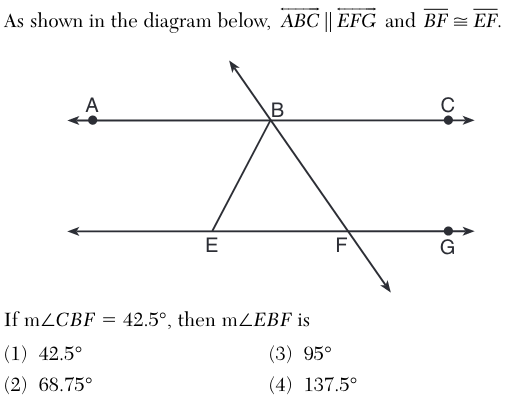
\includegraphics[width=0.6\textwidth]{4-9_transversal+isosceles.png}
 \\
 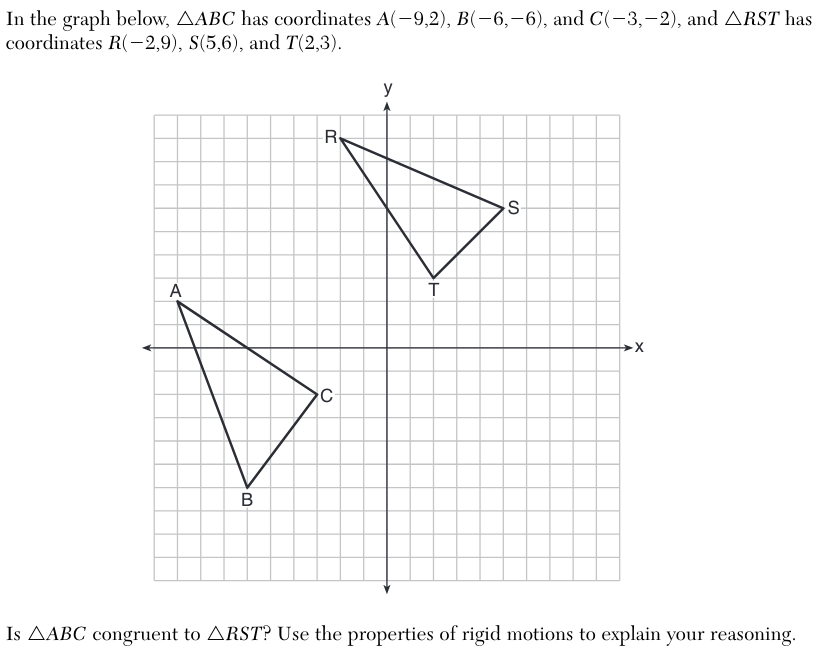
\includegraphics[width=1.0\textwidth]{4-9_reflection.png}


\end{enumerate}
\end{document}
